%!TEX root = ../Main.tex

\chapter{Assignment 3.3}

\textbf{Create 2 modules that realize a producer and a consumer thread. The modules should be
	connected together using a sc\_fifo channel. Use the structure of a TCP package to simulate the
	data transmitted over the transmission (fifo) channel. The producer transmits a new TCP package
	with a random interval between 2-10 ms. The consumer thread must print the simulation time and
	sequence number each time a new TCP package is received. Use the TCP Header structure as
	described below with a total package size of 512 bytes. Inspiration can be found in the FifoFilter
	(Fork.h, when adding two consumers) example project.
}

For this problem two modules are implemented; a Consumer and a Producer module. 
A code snippet of the Costumer module is snippet below. 
The consumer module implements sc\_fifo\_in of the type <TCPHeader> because its supposed to read from the FIFO.

\subsection{Consumer.h}
\begin{lstlisting}
#pragma once
#include <systemc.h>
#include "TCPHeader.h"

SC_MODULE(Consumer)
{
sc_fifo_in <TCPHeader*> in;
TCPHeader *header;
SC_CTOR(Consumer)
{
SC_THREAD(ConsumerThread);
}

void ConsumerThread(void);
};
\end{lstlisting}


\subsection{Producer.h}
The same goes for the Producer module just vise versa it implements sc\_fifo\_out of the type <TCPHeader> because it’s supposed to write to the FIFO. The code snippet of the Producer module header file is pictured below.
\begin{lstlisting}
#pragma once
#include <systemc.h>
#include "TCPHeader.h"

SC_MODULE(Producer)
{
sc_fifo_out <TCPHeader*> out;
SC_CTOR(Producer)
{
SC_THREAD(ProducerThread);
}

void ProducerThread(void);
};
\end{lstlisting}





\subsection{TCPHeader.h}
In the header file for TCPheader the code snippet from the exercise was used as a template for the structure of the TCPheader. The implementation can be seen below. Comments in the code explain the implementation.

\begin{lstlisting}
#pragma once
#include <systemc.h>
#define PACKET_SIZE 512
#define DATA_SIZE (PACKET_SIZE-20)

class TCPHeader
{
sc_uint<16> SourcePort;
sc_uint<16> DestinationPort;
sc_uint<32> SequenceNumber;
sc_uint<32> Acknowledge;
sc_uint<16> StatusBits;
sc_uint<16> WindowSize;
sc_uint<16> Checksum;
sc_uint<16> UrgentPointer;
char Data[DATA_SIZE];

public:

// Empty constrtuctor
TCPHeader()
{

}

// Parametrized constructor
TCPHeader(sc_uint<16> SourcePort, sc_uint<16> DestinationPort, sc_uint<32> SequenceNumber, sc_uint<32> Acknowledge, sc_uint<16> StatusBits, sc_uint<16> WindowSize, sc_uint<16> Checksum, sc_uint<16> UrgentPointer, char Data[DATA_SIZE])
{
this->SourcePort = SourcePort;
this->DestinationPort = DestinationPort;
this->SequenceNumber = SequenceNumber;
this->Acknowledge = Acknowledge;
this->StatusBits = StatusBits;
this->WindowSize = WindowSize;
this->Checksum = Checksum;
this->UrgentPointer = UrgentPointer;
strcpy(this->Data, Data);
}

sc_uint<32> getSequenceNumber()
{
return SequenceNumber;
}

void setSequenceNumber(sc_uint<32> sn)
{
SequenceNumber = sn;
}

// Overload of '='-operator.
// Creates a new instance with matching attributes.
TCPHeader& operator=(
const TCPHeader& rhs
)
{
SourcePort = rhs.SourcePort;
DestinationPort = rhs.DestinationPort;
SequenceNumber = rhs.SequenceNumber;
Acknowledge = rhs.Acknowledge;
StatusBits = rhs.StatusBits;
WindowSize = rhs.WindowSize;
Checksum = rhs.Checksum;
UrgentPointer = rhs.UrgentPointer;
strcpy(Data, rhs.Data);
return *this;
}
// Overload of '=='-operator.
// Checks if all values are the same, in which case true is returned. Otherwise false is returned.
bool operator==(const TCPHeader& rhs)
const {
return SourcePort == rhs.SourcePort
&& DestinationPort == rhs.DestinationPort
&& SequenceNumber == rhs.SequenceNumber
&& Acknowledge == rhs.Acknowledge
&&StatusBits == rhs.StatusBits
&&WindowSize == rhs.WindowSize
&&Checksum == rhs.Checksum
&&UrgentPointer == rhs.UrgentPointer
&&strcmp(Data, rhs.Data);
}


//Definition of '<<'-operator and sc_trace.
friend ostream& operator<<(ostream& file, const TCPHeader& trans);
friend void sc_trace(sc_trace_file*& tf, const TCPHeader& trans, std::string nm);
};
\end{lstlisting}


\subsection{Producer.cpp}

If we look at the source file for the Producer which is pictured below. 
It generates a new TCPHeader called header, and write information about the package to the console, before writing the package to the FIFO. Then the sequence number is incremented before it waits for a random amount of time (between 2ms and 10ms). 

\begin{lstlisting}
#include "Producer.h"

sc_uint<16> SourcePort =  1;
sc_uint<16> DestinationPort = 2;
sc_uint<32> SequenceNumber = 1;
sc_uint<32> Acknowledge = 4;
sc_uint<16> StatusBits = 5;
sc_uint<16> WindowSize = 6;
sc_uint<16> Checksum = 7;
sc_uint<16> UrgentPointer = 8;
char Data[DATA_SIZE] = "Test Data";

void Producer::ProducerThread(void)
{
TCPHeader *header;
while (1)
{
// Generate new TCP header.
header = new TCPHeader(SourcePort, DestinationPort, SequenceNumber, Acknowledge, StatusBits, WindowSize, Checksum, UrgentPointer, Data);
cout << sc_time_stamp() << ": Producing" << endl;
cout << "Sending: " << endl << *header << endl << endl;

//Write to FIFO
out.write(header);

// Increment sequence number.
SequenceNumber++;

// Wait for 2-10 ms.
int waitTime = rand() % 10 + 2;
wait(waitTime, SC_MS);
}
}
\end{lstlisting}



\subsection{Consumer.cpp}
The consumer just reads from the FIFO, and writes out the sequence number on the received package to the console. 
\begin{lstlisting}
#include "Consumer.h"
#include "TCPHeader.h"

void Consumer :: ConsumerThread(void)
{
while (1)
{
// Blocking read from FIFO
header = in.read();
// Output timestamp and info about TCP package.
cout << sc_time_stamp() << " - Received TCP Package - Sequence number: " << (*header).getSequenceNumber() << endl << endl;
}
}$ 	 $
\end{lstlisting}



Below is a picture of the simulated result from the console. 
It matches the expected result. The sequence numbers match and the packages are being send in a random interval between 2ms and 10ms. 


\begin{figure}[H]
	\centering
	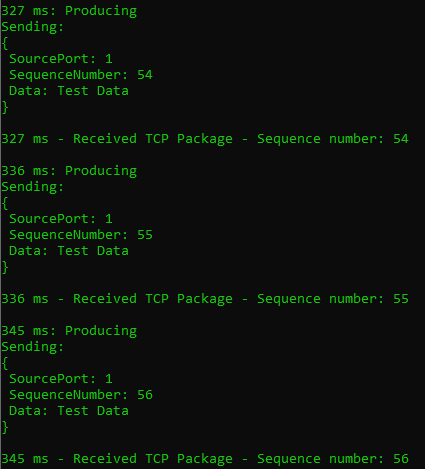
\includegraphics[width=\textwidth]{Images/ConsoleWindow3_3.png}
	\caption{A screenshot of the console}
	\label{fig:ConsoleWindow_3_3}
\end{figure}


\section{Assignment 3.3.2}

\textbf{The producer must be rewritten to connect to more ports. As illustrated below:}
	
\begin{lstlisting}
sc_port<sc_fifo_out_if<TCPHeader *>,0> out;
\end{lstlisting}
	
\textbf{Further, the producer code must be rewritten to send the TCP packet to all connected fifo channels as
shown below:}

\begin{lstlisting}	
for (int i = 0; i < out.size(); i++)
{
out[i]->write(package);
}
\end{lstlisting}

In this exercise its only the header file for the Producer and the two source files for Producer and Consumer that has changes the rest is identical to the previous exercise. 

\subsection{Producer.h}
If we look at the Producer.h. The only thing that has changed is line 7, it is now possible for the producer to connect to five ports.

\begin{lstlisting}
#pragma once
#include <systemc.h>
#include "TCPHeader.h"

SC_MODULE(Producer)
{
sc_port<sc_fifo_out_if<TCPHeader*>, 5> out;
SC_CTOR(Producer)
{
SC_THREAD(ProducerThread);
}

void ProducerThread(void);
};
\end{lstlisting}



\subsection{Producer.cpp}
The Producer.cpp hasn't changed mush either. Its now running a for-loop to make sure it writes to all its connected ports. 
\begin{lstlisting}
#include "Producer.h"

sc_uint<16> SourcePort =  1;
sc_uint<16> DestinationPort = 2;
sc_uint<32> SequenceNumber = 1;
sc_uint<32> Acknowledge = 4;
sc_uint<16> StatusBits = 5;
sc_uint<16> WindowSize = 6;
sc_uint<16> Checksum = 7;
sc_uint<16> UrgentPointer = 8;
char Data[DATA_SIZE] = "Test Data";

void Producer::ProducerThread(void)
{
TCPHeader *header;
while (1)
{
header = new TCPHeader(SourcePort, DestinationPort, SequenceNumber, Acknowledge, StatusBits, WindowSize, Checksum, UrgentPointer, Data);


//Write to FIFO
for (int i = 0; i < out.size(); i++)
{
// Generate new TCP header.
cout << sc_time_stamp() << ": Producing" << endl;
header->setDestinationPort(i + 1);
cout << "Sending: " << endl << *header << endl << endl;

out[i]->write(header);
}

SequenceNumber++;

// Wait for 2-10 ms.
int waitTime = rand() % 10 + 2;
wait(waitTime, SC_MS);
}
}
\end{lstlisting}



\subsection{Consumer.cpp}
Again the Consumer.cpp hasn't changed mush either. The main difference is the consumer now has to keep track of the process which is done in line 7.
\begin{lstlisting}
#include "Consumer.h"
#include "TCPHeader.h"

void Consumer :: ConsumerThread(void)
{
//To get the current process name
const char* processName = sc_core::sc_get_current_process_b()->get_parent()->basename();
while (1)
{
header = in.read();
cout << sc_time_stamp() << " - " << processName << " received TCP Package - Sequence number: " << (*header).getSequenceNumber() << endl << endl;
if (strcmp(processName,"consumer_2")==0)
{
delete header;
}

}
}
\end{lstlisting}

In main.cpp two FIFO channels, one producer and two consumers where created and the simulation time was 120ms. Below is a picture of the simulation result from the console window to show the producer sends data to both consumers. 


\begin{figure}[H]
	\centering
	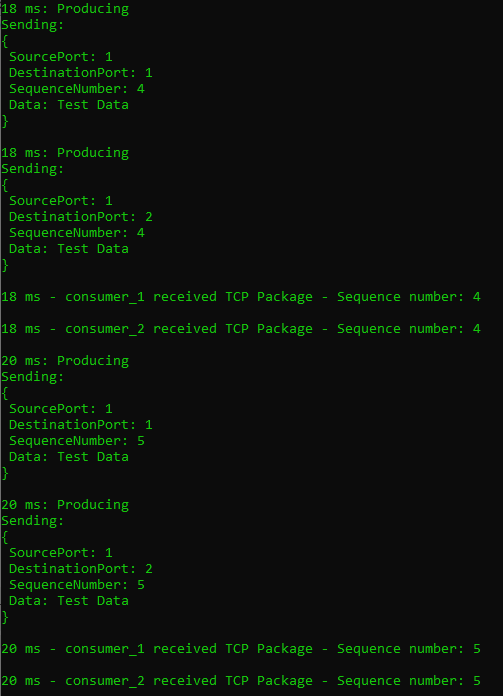
\includegraphics[width=\textwidth]{Images/ConsoleWindow3_3_2.png}
	\caption{A screenshot of the console}
	\label{fig:ConsoleWindow_3_3_2}
\end{figure}



